
\documentclass[a4paper,12pt]{report}
%    \renewcommand{\baselinestretch}{1.6}      % interline spacing
%
% \includeonly{}
%
%			PREAMBOLO
%
\usepackage[a4paper]{geometry}
\usepackage{amssymb,amsmath,amsthm}
\usepackage{graphicx}
\usepackage{url}
\usepackage{hyperref}
\usepackage{epsfig}
\usepackage[italian, english]{babel}
\usepackage{setspace}
\usepackage{style}
\graphicspath{ {./img/} }
\usepackage{float}
\usepackage{booktabs}

\usepackage{wrapfig}
% per le accentate
\usepackage[utf8]{inputenc}
%
\newtheorem{myteor}{Teorema}[section]
%
\newenvironment{teor}{\begin{myteor}\sl}{\end{myteor}}
%
%
%			TITOLO
%
\begin{document}

  

\title{Cloud Gaming}
\author{Daniele Bocchino}
\anno{2021-2022}
\matricola{991031}
\relatore{Prof. Gianini Gabriele}


\beforepreface
\afterpreface
%
%
%			
\chapter{Introduction}
\label{cap1}
%
%
\section{Cloud Gaming}
During the Covid-19 pandemic of 2020, a lot of people were forced to stay at home for several month and  a lot of them looked for a different way to spend their time. New people have entered the world of video games and they tried to purchase the best solution for playing games. Unfortunately due to the chip crisis and production slowdowns caused by the pandemic to purchase a console or built PC games had became a titanic challenge. For this reason a lot of people has opted for cloud-based solutions to play major video game titles.\\
%
\section{History of Cloud Gaming}
The first approach of cloud gaming technology sates back to the early 2000s. For several years this technology didn't explode due by lower connection performance  and other problems. Recently, after explosion of various SaaS ( Software as a Service ) such as Netflix, and access to a fast internet connection for many people, more and more companies have wanted to invest in the cloud-based gaming. Large Company such as Google, Amazon, Microsoft, Nvidia, Shadow, etc... Have invested in the possibility of playing video games in the cloud.\\
\newpage
%
\section{How could gaming really works?}
Cloud gaming allows users to play online games through remote hardware owned by a cloud provider. Instead of players inserting a game disc into a gaming console or downloading a game’s file to their device, players stream games via the web.\\
This solution allow anyone with a good connection to play the best games in the world ( the classic games called AAA ) with any type of device that can be connected to the internet.\\\\
The idea is really great, allowing gamers not to buy a specific device and play the best games on smartphones, tablets or computers without incredible performance. \\
%
Cloud gaming platforms works as a remote desktop. The games are stored and executed on remote computer, and then streamed on the player's device. In many case, users are required to download a specific application or navigate to a dedicated web page to start playing games. Through this method the users don't have to worry about downloading games, updating it or upgrading hardware. This operation are managed by service provider.\\\\
%
In addition to taking care of the hardware, the service provider also takes care of adding new games; in fact, a different cloud games provider offers a monthly subscription that includes a library with some available games. In general this game are of different types and popularity.\\
%
\subsection{Advantages of Cloud Gaming}
The cloud gaming has brought a plethora of benefits to users and the gaming world, first and foremost the ability to play a large number of titles without  expensive hardware and on any type of devices. Other advantages are related to the ability to try a lot of games without purchasing them and reduce time it takes users to update and download the games. In fact, to play on cloud, users need nearly 20 Mb/s download connection ( this value depends on the desired image resolution and the type of service provider). At this speed, it may take several hours to download the game. 
\newpage
%
\subsection{Disadvantages of Cloud Gaming}
Cloud gaming doesn't only have advantages, with this immature technology there are some disadvantages that may disappoint the most demanding gamers. The main problem with this type of gaming is the connection, although many people connect with a very fast internet ( the famous gigabit connection ) this type of technology depends on latency. In fact in many cases, the very fast internet connection is not enough for a great cloud gaming experience. For this reason in a lot of games that the timing and precision of the users input is mandatory for obtain a really good experience ( such as First-person shooters and fighting games ) will not work as a local machine and the user experience will be sacrificed. Another disadvantage is related to the game library, a problem that depends on the service provider and the relationship between the service provider and game companies. It may indeed be the case that a recent game needs a few months before it becomes available on the on-demand library, or it is possible that a game will never be available. 
 %
\chapter{Process}
\label{cap2}
\section{The Users}
As in any business, everything revolves around the customers, Cloud Gaming was created for them, to offer a viable alternative to traditional gaming.\\
It is a great solution for off-site students, commuters and all those people who do not need very high performance with some small sacrifice. \\
To use the service, users must register and pay a monthly subscription.Depending on the cloud gaming service provider, users can use the service on the web browser or on a dedicated application.\\
After logging in, users can choose the game they want and start it.\\
If the user wishes, they can stop the subscription at any time and reactivate it whenever they want. \\
Within the project the user is also allowed to report inefficiencies or functional bugs within the games or platform.\\
This provides a way for the user to submit reports so as to improve the service received. 

\newpage
%
\section{The Cloud computing Company }
A cloud computing company is a company that develops a service to allow users to play a large number of games.\\
This is done by providing enough high-performance hardware to support the load of users and fully enjoy the service.\\
This service is usually a platform where users can log on and start a game from those within the company's servers.\\
This company includes different types of workers. In this project, the part of the company providing the service is assumed to include:
\begin{itemize}
\item{\textbf{The cloud gaming service:}the platform with which users interact;}
\item{\textbf{The financial \& Management team:} which is responsible for managing the budget and making strategic choices;}
\item{\textbf{The cloud gaming service:} employed in maintaining the hardware and software of the cloud computing service.}
\end{itemize}
%
\subsection{The cloud gaming service }
The cloud gaming service is the platform for users to interact with. On it are all the available games and the ability to play them. \\
At access is required a registration by the user, then it is possible to subscribe to use the service. 
%  
\subsection{The engineering team }
The engineering team is a group of people who work with the machines. In general, this team monitors machine, fix problem, make upgrade to hardware, manage all dates inside the cloud etc... \\
They are in charge of making the games available in the cloud after receiving them from the manufacturing companies following the agreements between the two parties.
%
\subsection{The financial and Management team }
The finance and management team is a group of people who interface with game companies. Their role is to define market strategies, evaluate the only asset, and define an appropriate business plan to ensure growth and profit for the company. In addition to this they are tasked with discussing with game companies, making requests on new titles, and obtaining permission to distribute the game on the cloud platform in exchange for payment. 
%
\section{The video game company }
A video game company is a company that creates video games. Often these titles are only available on certain platforms or devices (such as console exclusives). In the specific case examined by this project, the video game company interfaces with the company that provides a cloud computing service to make its products available on the cloud game library. This company is composed of several departments working in unison to generate a satisfactory product. In this project, it is assumed that the company comprises only two departments:
\begin{itemize}
\item{\textbf{The Development Department:} which includes a large number of employees such as : developers, designers designers etc...}
\item{\textbf{The Release \& Management Department:} containing both the finance team that defines market strategies and interfaces with the company in the cloud, and the release team that is responsible for providing a final evaluation before deploying the product .}
\end{itemize}
%
\subsection{Development Department }
It is the department of a video game company that takes care of the development part of a new game through various figures in charge of the graphics, the code part, and the design part. In addition to this, it also deals with the creation of new features and fixing structural bugs in the video game.
%
\subsection{Release and Management Department }
It is the department in a video game company that deals with the release part of a new game and the establishment of financial strategies in order to ensure economic stability for the company. It interfaces with the finance and management team of the company that runs the cloud computing service. Its job is to sell the product to the cloud computing company at the best price and then provide the engineering team with the product to be included in the on-demand library. The release part, on the other hand, is also in charge of verifying the title before it is launched in the market.
%
%
\chapter{Business Process Flow}
\section{BPMN - Business Process Model and Notation Diagram }
Business Process Model and Notation (BPMN) is a graphical representation for specifying business processes in a business process model.\\
Business Process Model and Notation(BPMN) is a standard for business process modeling that provides a graphical notation for specifying business processes in a Business Process Diagram (BPD).\\
The objective of BPMN is to support business process management, for both technical users and business users, by providing a notation that is intuitive to business users, yet able to represent complex process semantics.\\

\subsection{Structure of BPMN}
BPMN. As stated earlier, a business process involves events and activities.
\begin{itemize}
\item{\textbf{Events:} represent things that happen instantaneously (e.g. an invoice has been received). Events are represented by circles, activities by rounded rectangles, and arcs (called sequence}
\item{\textbf{Activities:}  represent units of work that have a duration (e.g. an activity to
pay an invoice). Activities by rounded rectangles}
\item{\textbf{Arcs:} in a process, events and activities are logically related. This relation will be created by arcs. The most elementary form of relation is that of sequence, which implies that one event or activity  is followed by another event or activity. Arcs are represented by arrows with a full arrow-head.}

\end{itemize}

\section{Full Diagram}
\begin{figure}[H]
 \centering
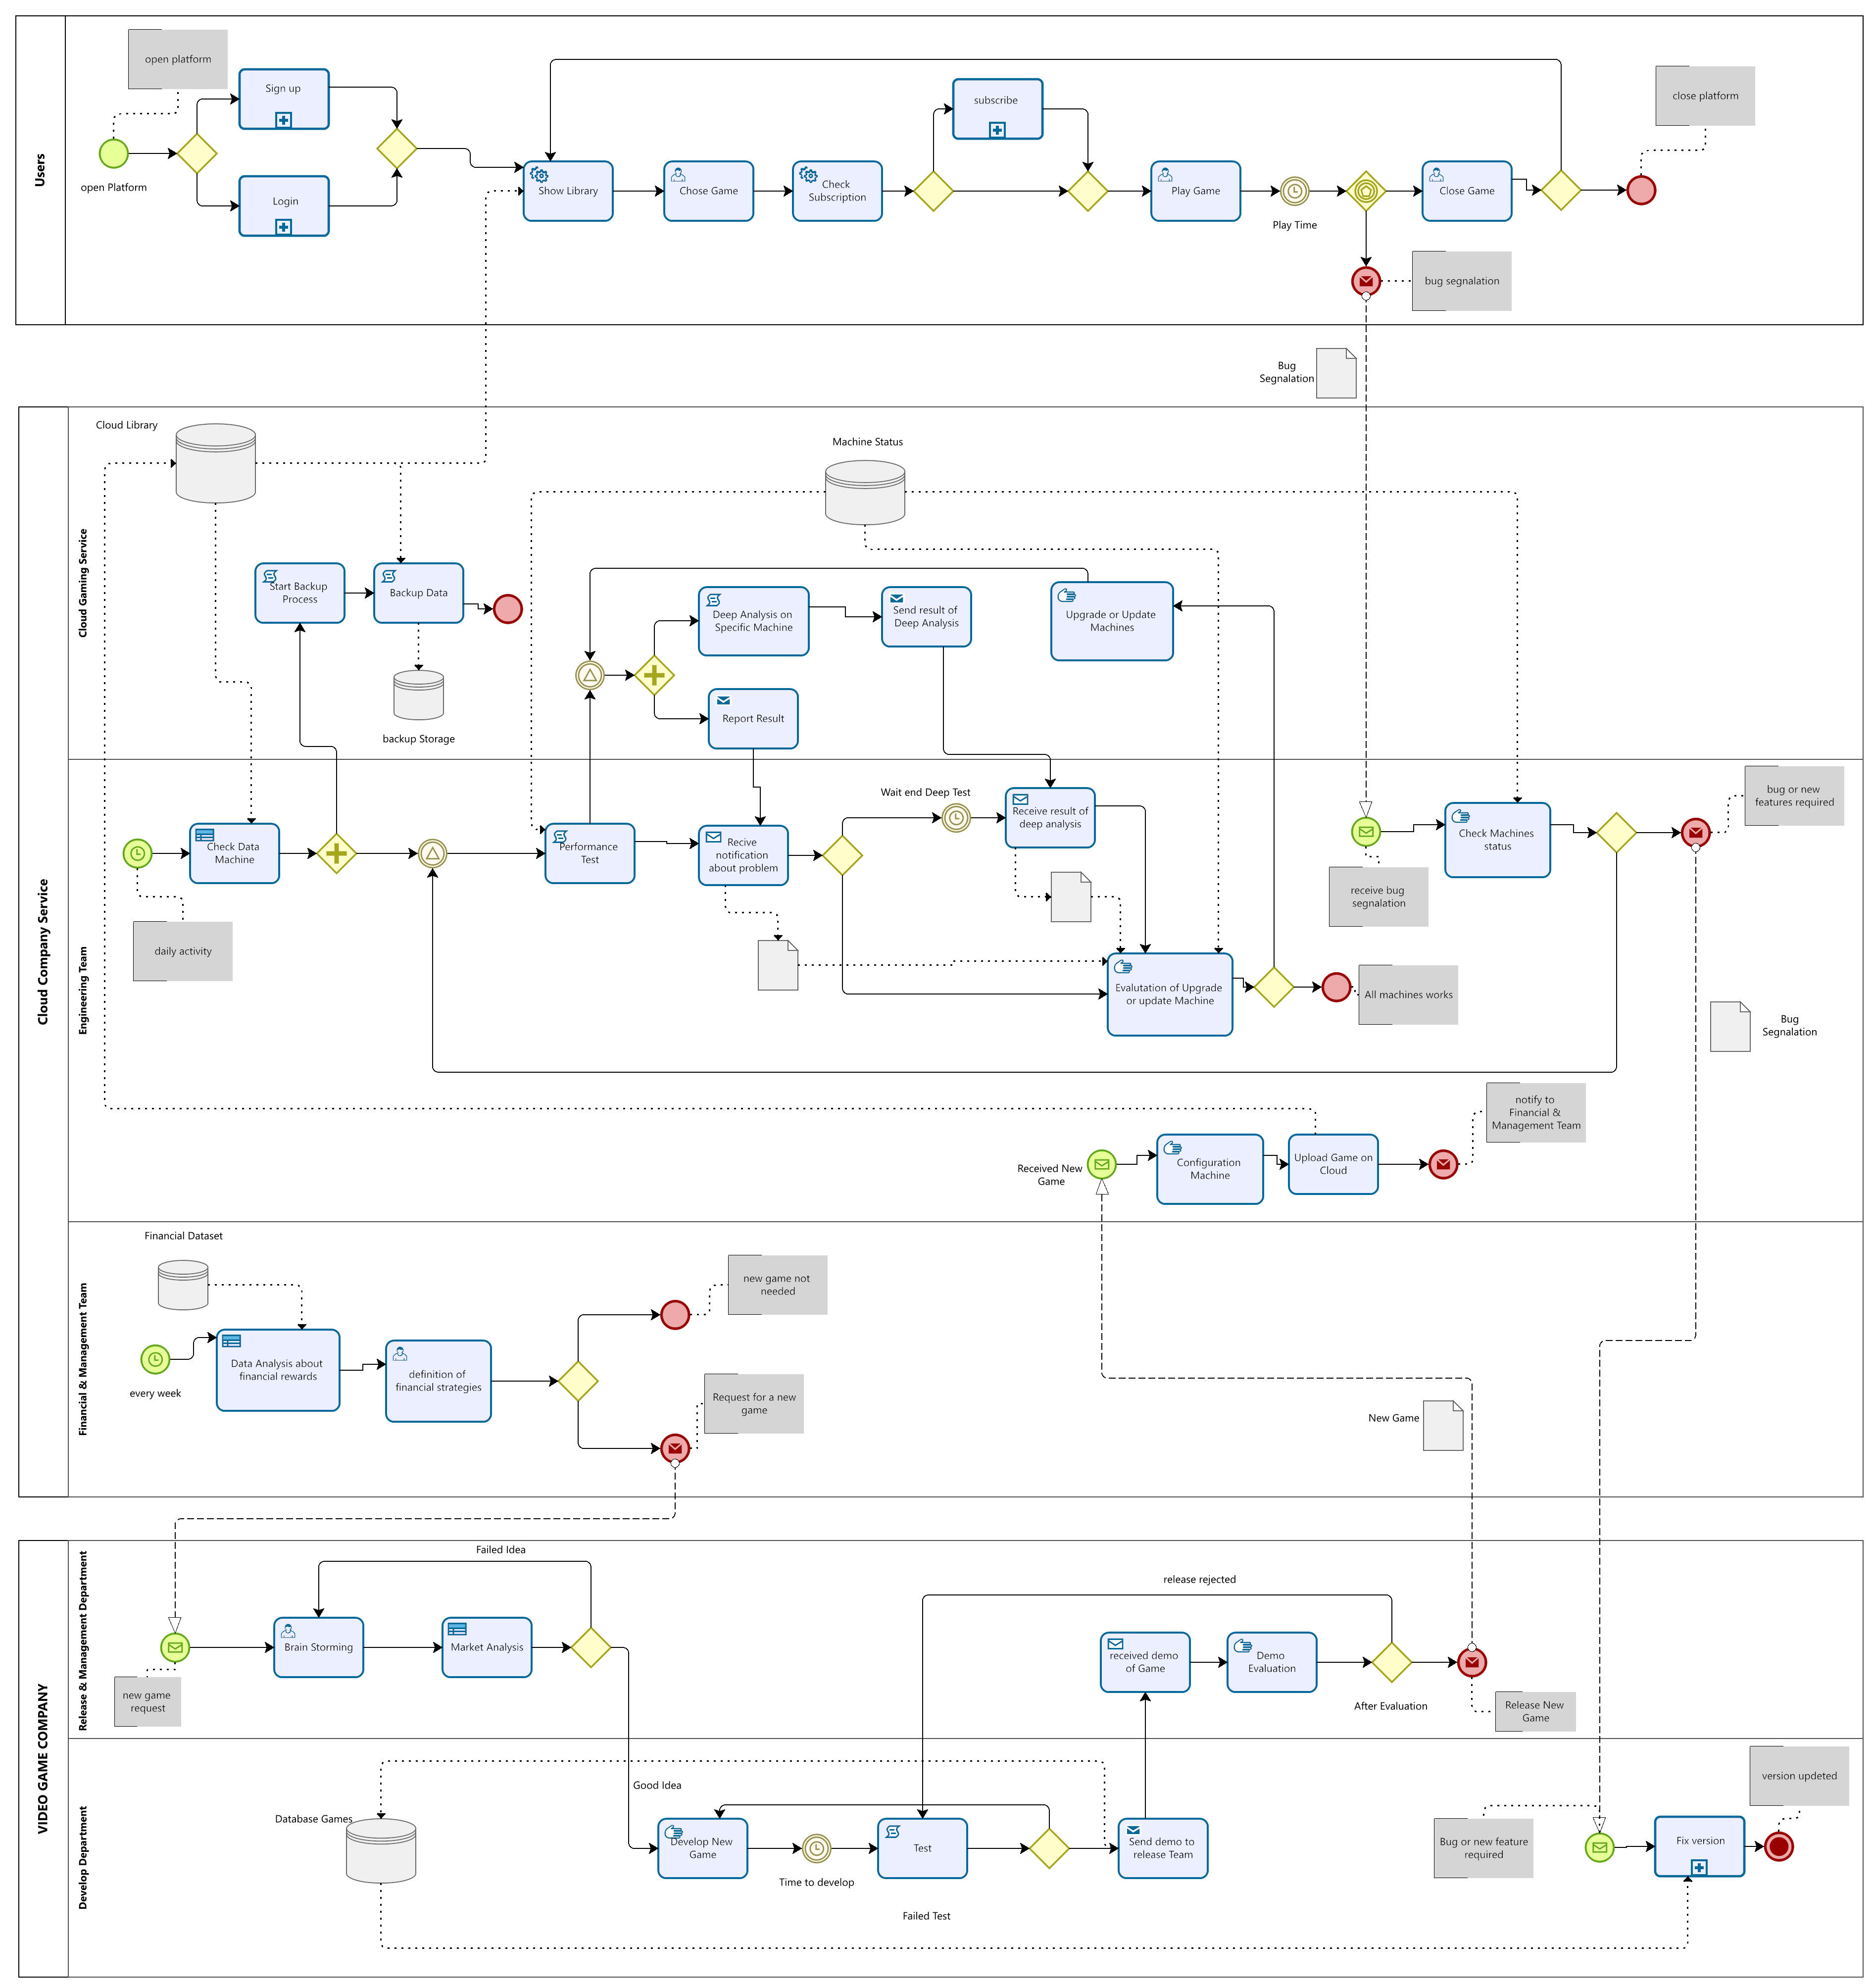
\includegraphics[scale=0.15]{Full_BPMN}
\caption{Full BPMN Diagram}
\label{FULL BPMN}
\end{figure} 
%
%
\section{The Users}
\begin{figure}[H]
 \centering
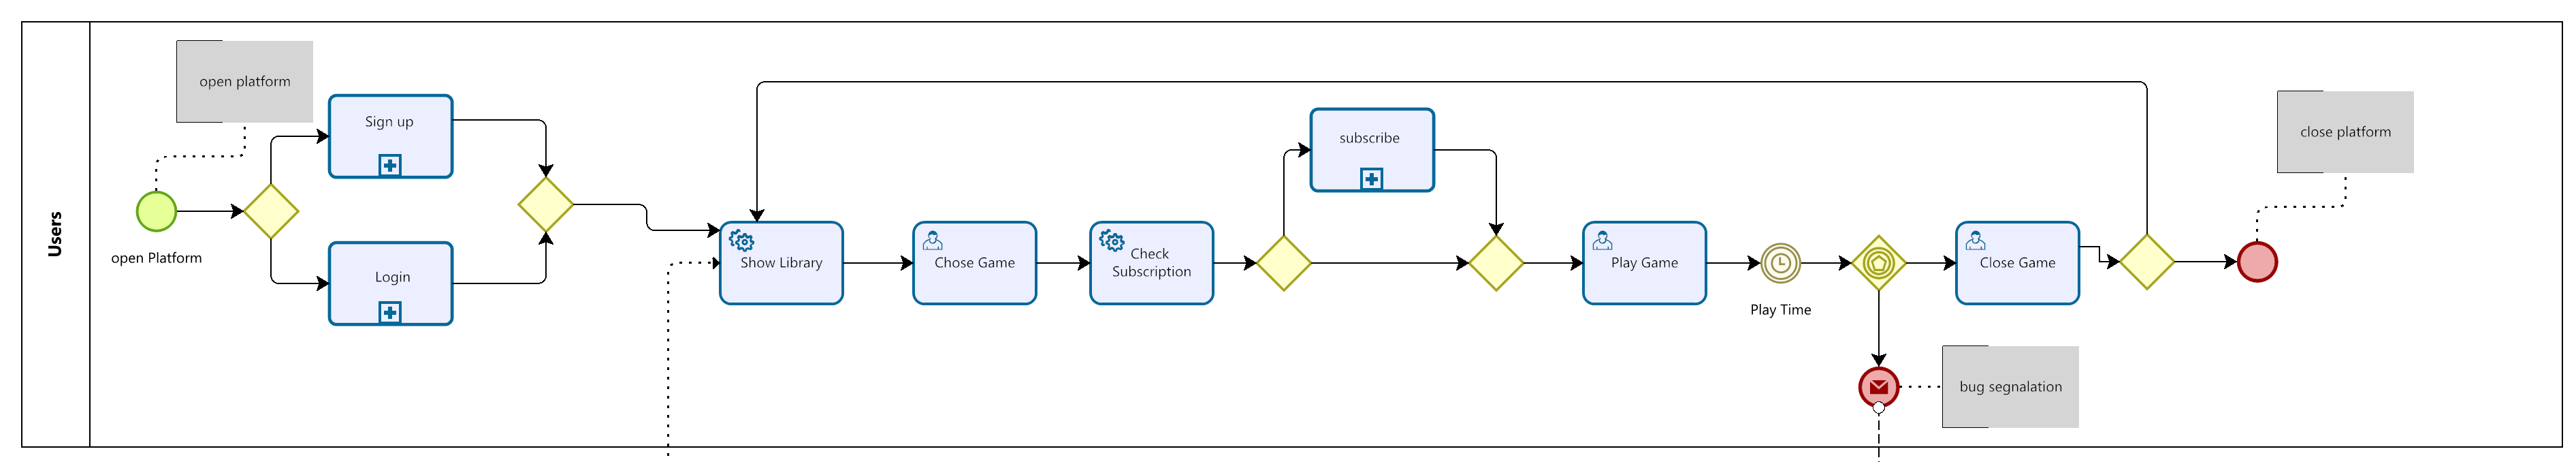
\includegraphics[scale=0.16]{user_BPMN}
\caption{Users BPMN Diagram}
\label{Users BPMN}
\end{figure} 

\subsection{Sub Process - Login }
\begin{figure}[H]
 \centering
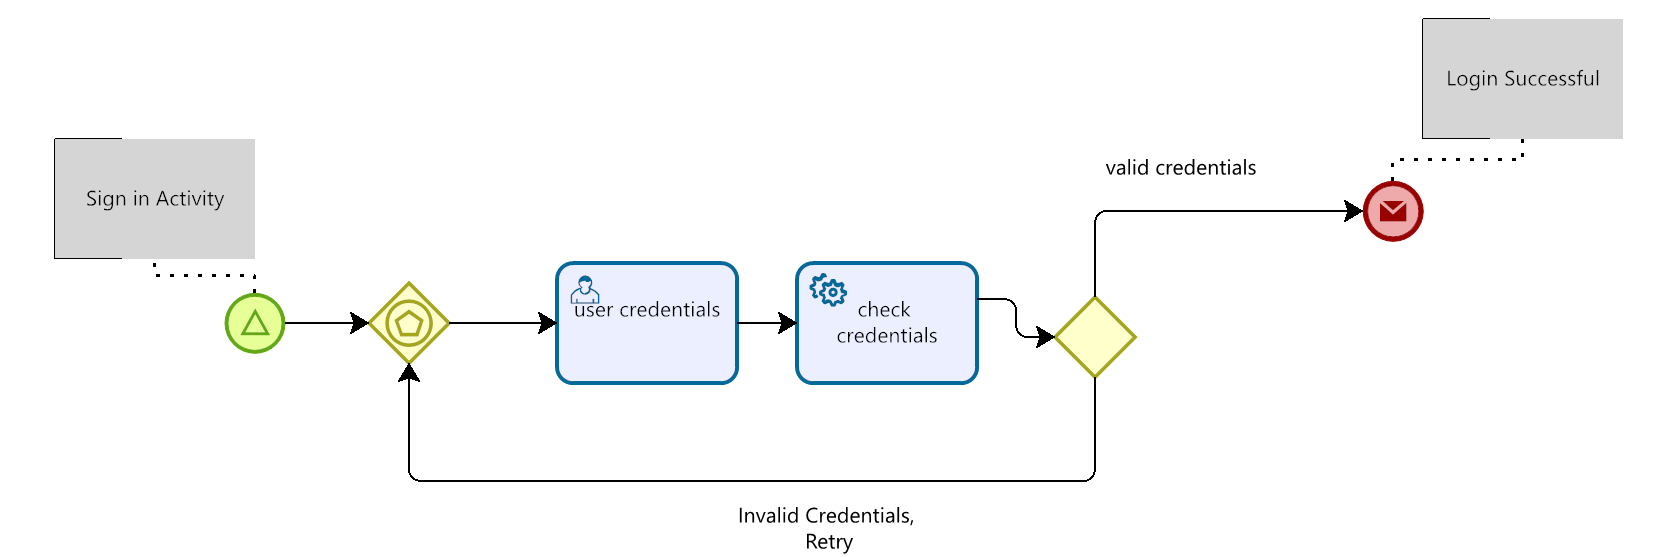
\includegraphics[scale=0.35]{login_BPMN}
\caption{Sub Process - Login BPMN Diagram}
\label{Login BPMN}

\end{figure} 

\subsection{Sub Process - Register }
\begin{figure}[H]
 \centering
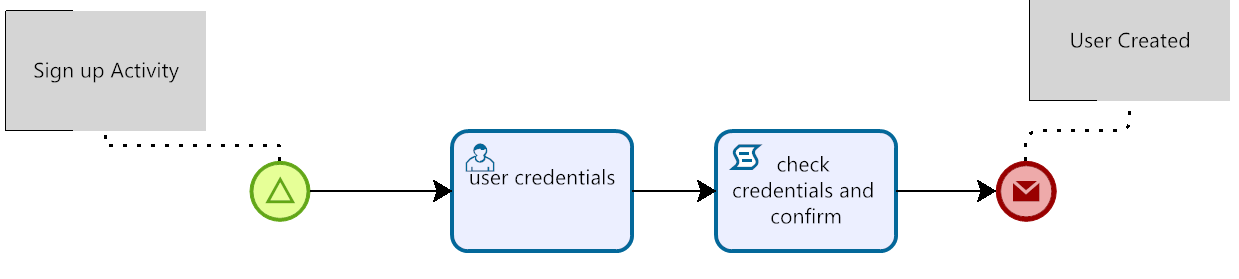
\includegraphics[scale=0.35]{signup_BPMN}
\caption{Sub Process - Sign up BPMN Diagram}
\label{Signup BPMN}
\end{figure} 

\subsection{Sub Process - Subscription }
\begin{figure}[H]
 \centering
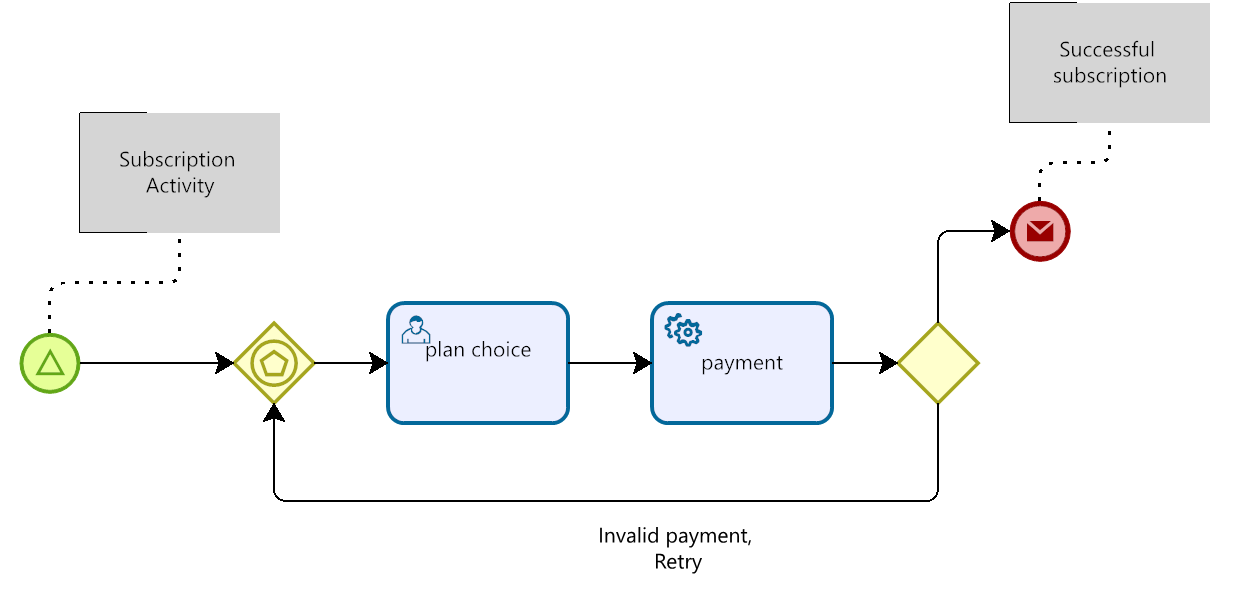
\includegraphics[scale=0.35]{subscription_BPMN}
\caption{Sub Process - Subscription BPMN Diagram}
\label{Subscription BPMN}
\end{figure} 

\section{The Cloud Computing service }
\begin{figure}[H]
 \centering
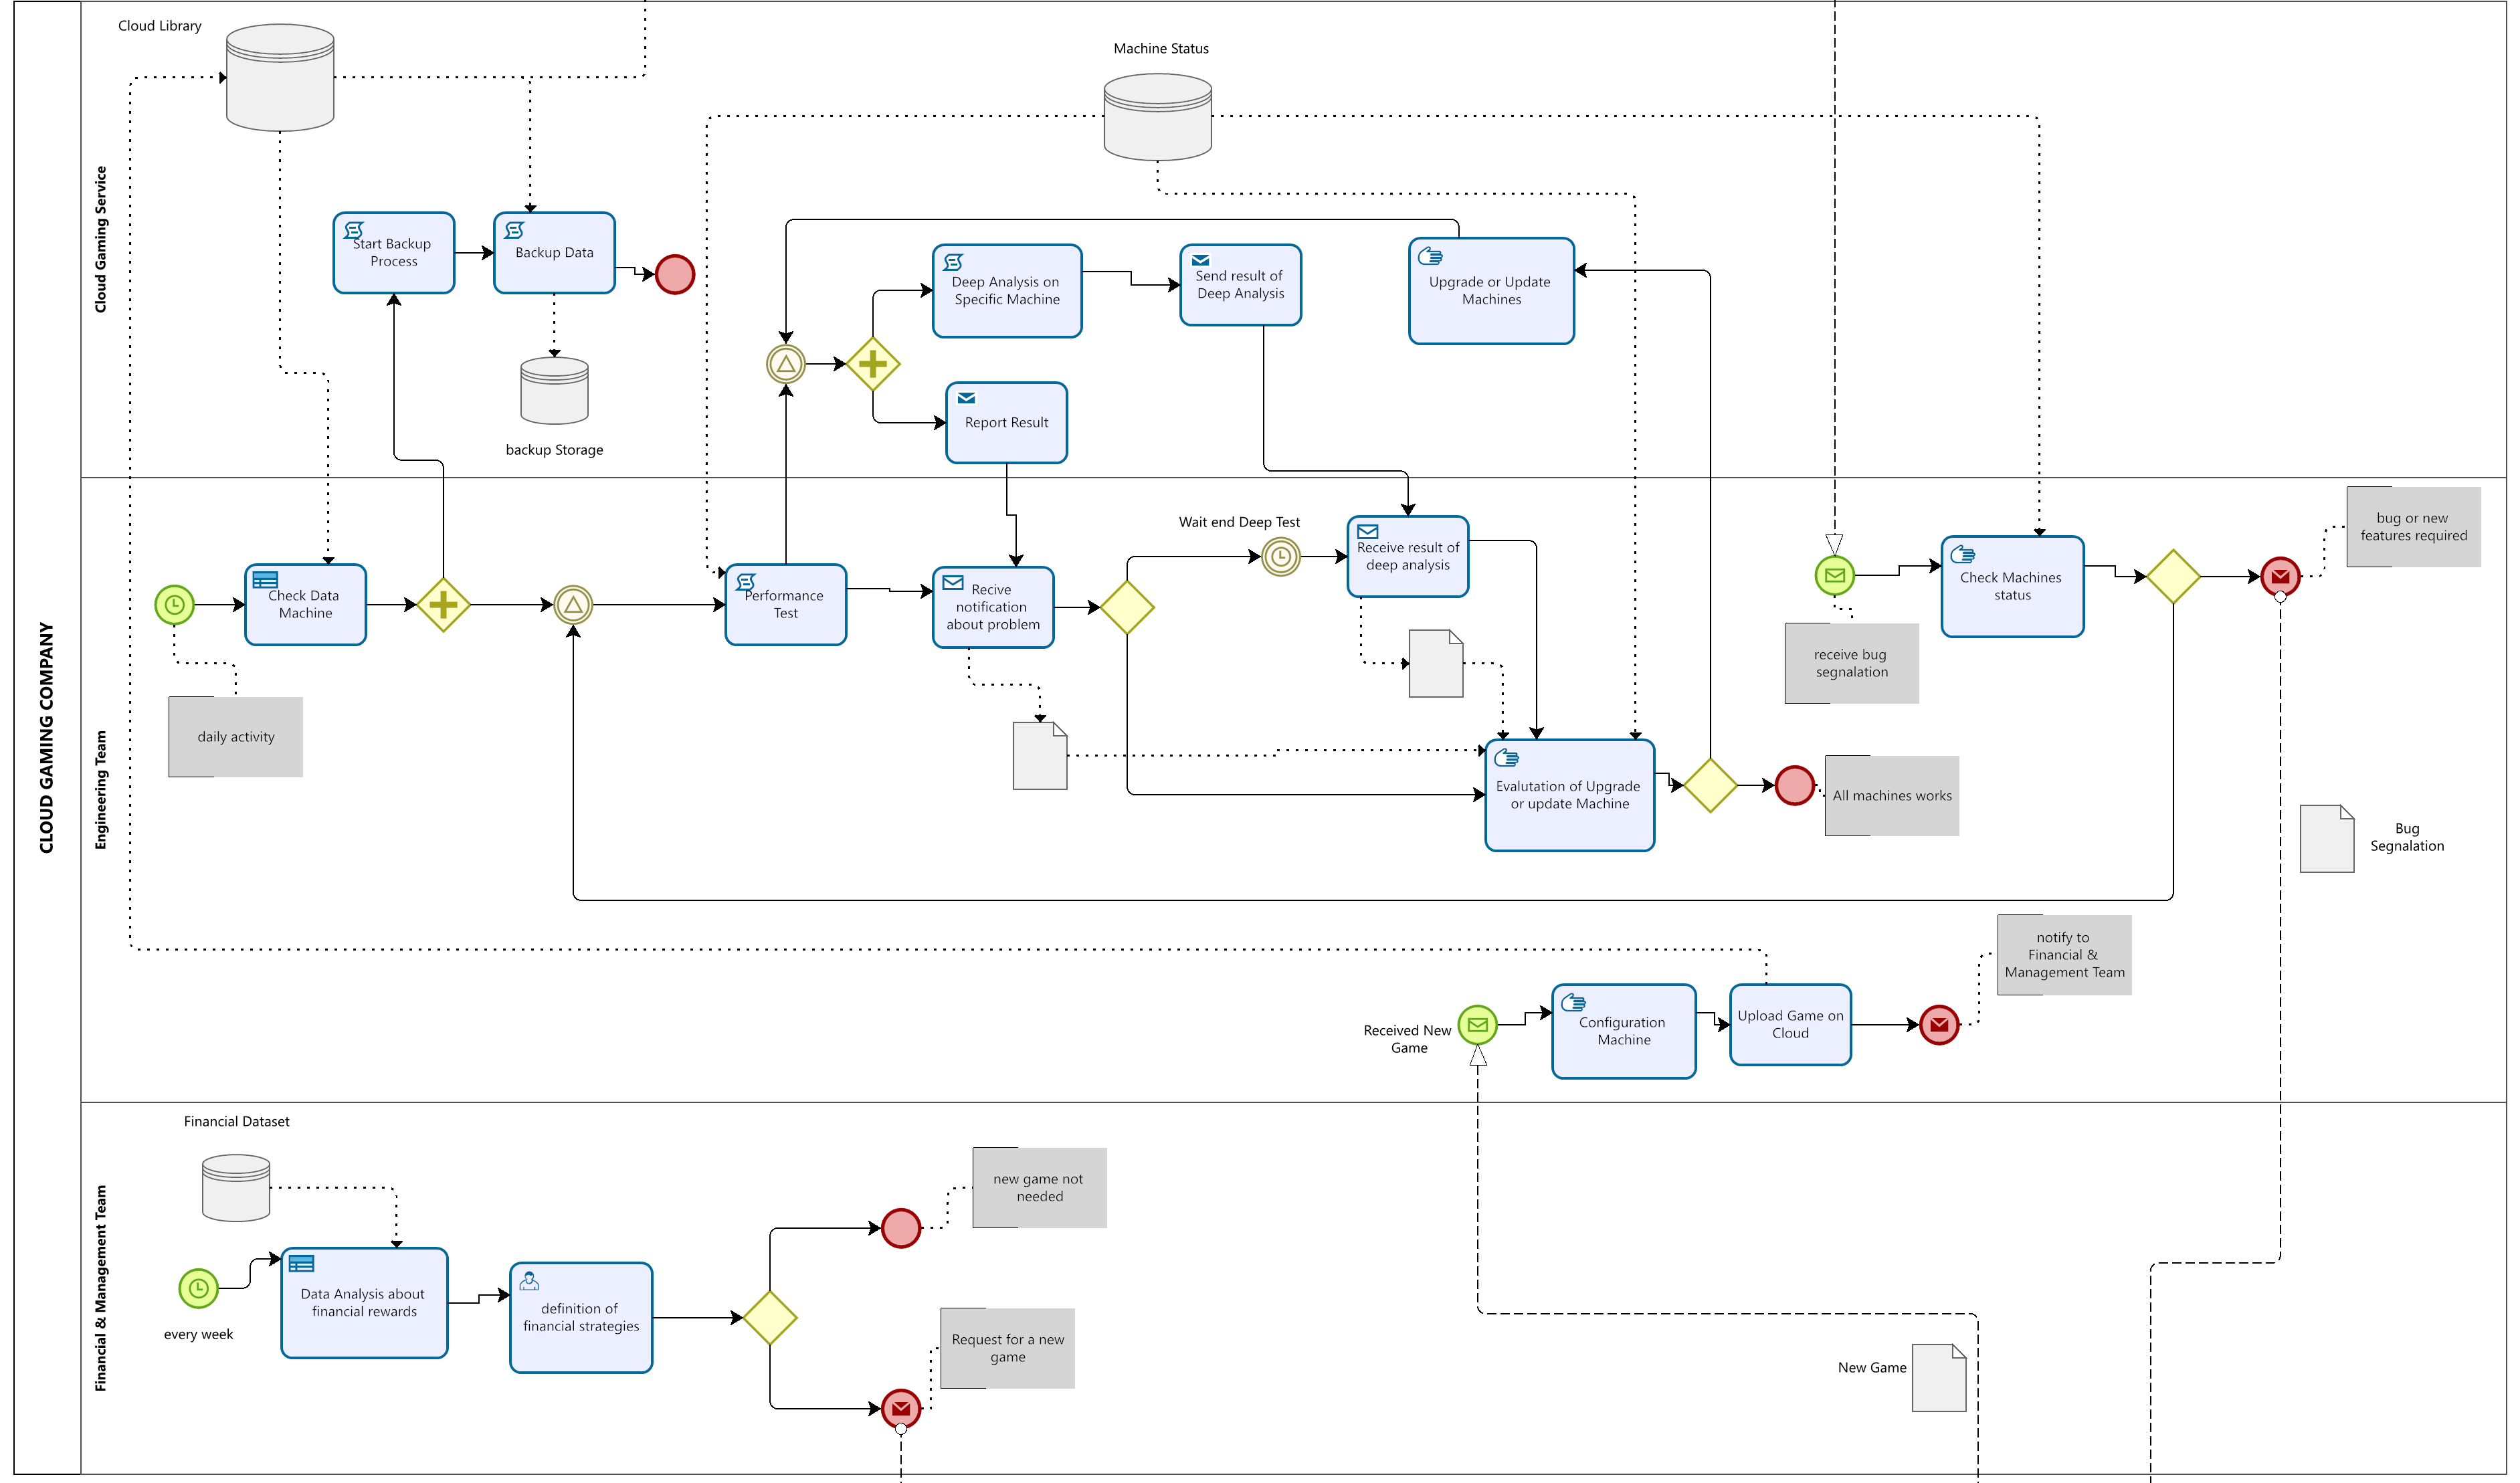
\includegraphics[scale=0.15]{cloud_BPMN}
\caption{Cloud Computing Service BPMN Diagram}
\label{Cloud BPMN}

\end{figure}



\section{The video game company  }
\begin{figure}[H]
 \centering
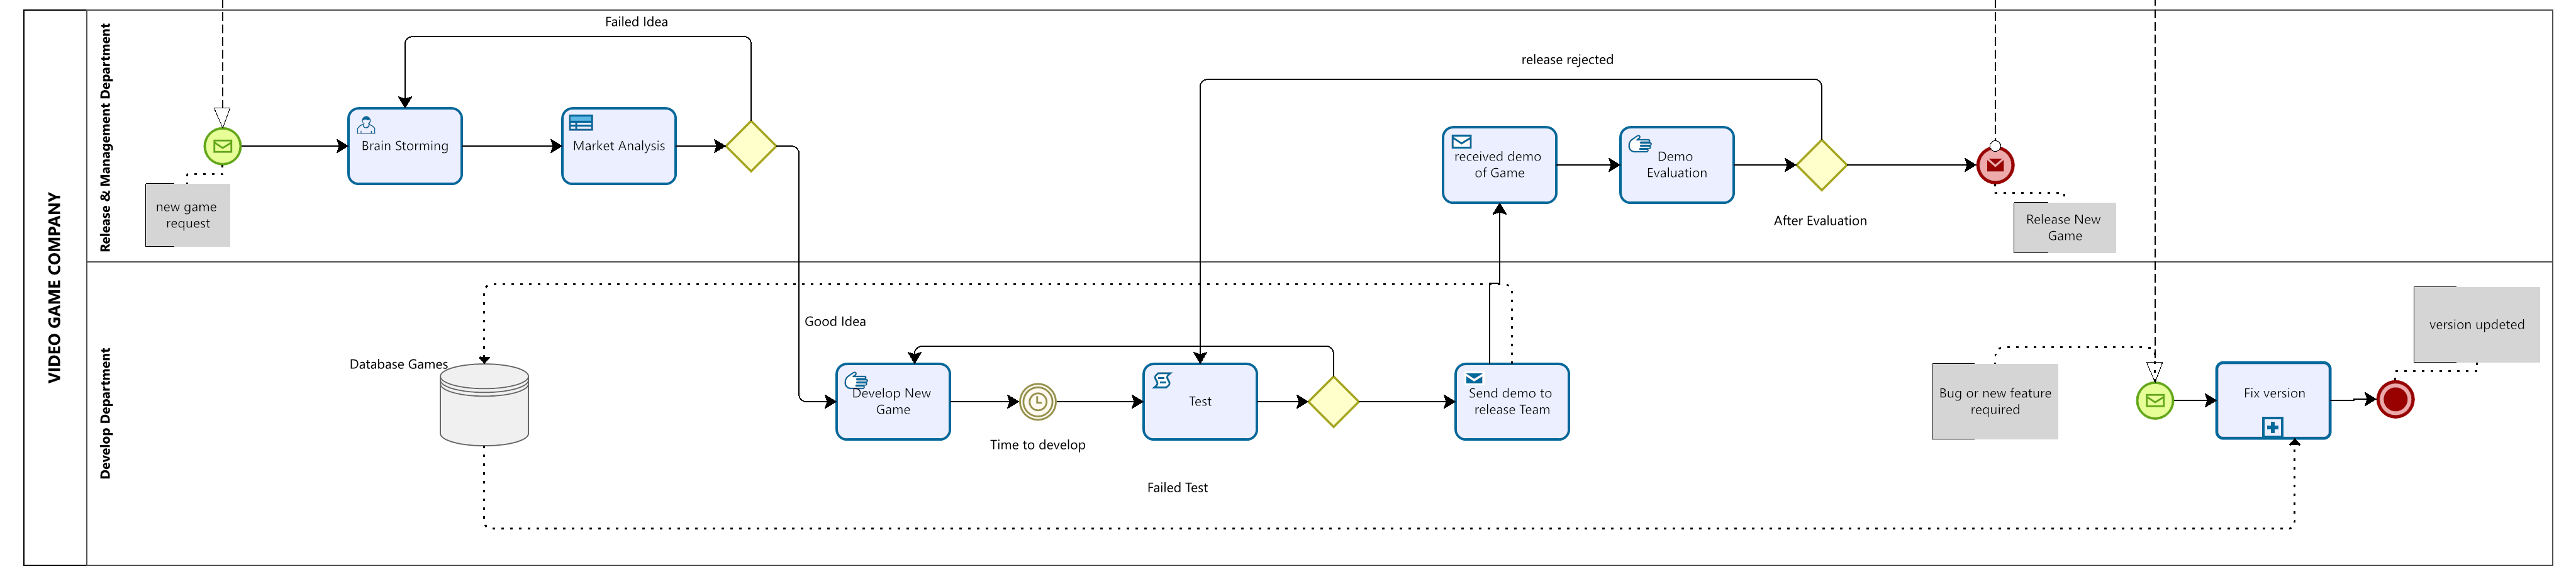
\includegraphics[scale=0.15]{videogame_BPMN}
\caption{Video Game Company BPMN Diagram}
\label{VideoGame BPMN}
\end{figure} 

\subsection{Sub Process - Fix Version }
\begin{figure}[H]
 \centering
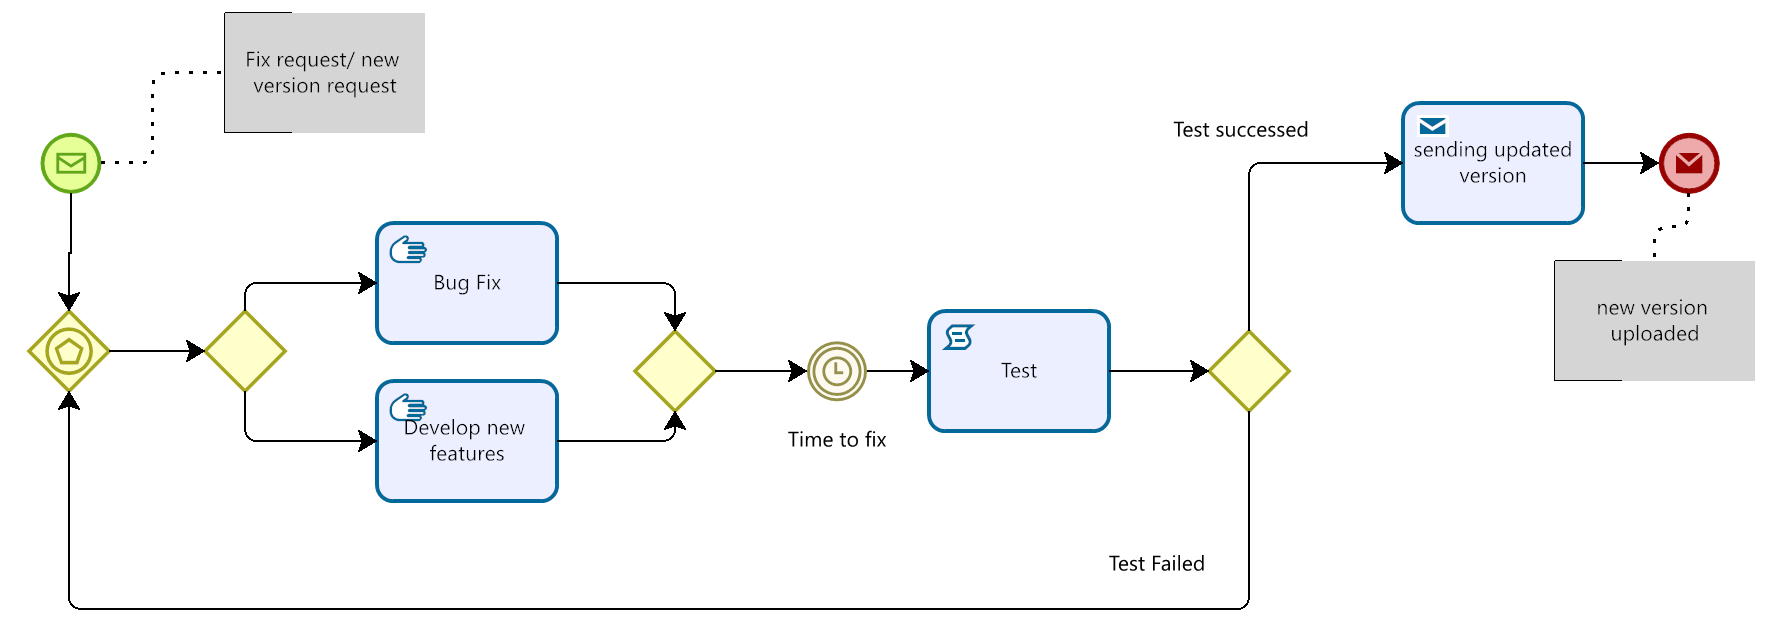
\includegraphics[scale=0.35]{developer_BPMN}
\caption{Sub Process - Fix Version BPMN Diagram}
\label{Fix Version BPMN}

\end{figure} 

\chapter{Value Model}
The Value Model describes what constitutes value in an organization, where organizations create value, how stakeholders exchange value, and, most importantly, how an organization can find new opportunities to create value.\\
A Value Model is basically a diagram designed to represent the exchange of services and payments
between different actors and/or market segments. In most cases there is no way to get
this diagram somehow, it has to be created from scratch.

\subsection{Structure of Value Model}
\begin{itemize}
\item{\textbf{Actor:} is an economically independent entity. It is represented by a square}
\item{\textbf{Value Exchange:} connects two Value Ports with each other. It is represented by lines}
\item{\textbf{Value Interface:} groups an input/output Value Ports. It is atomic.}
\item{\textbf{Value Ports:} is used by an actor to provide or request Value Objects to and from other
actors. It is an abstraction of internal business processes and can be an incoming input or output.}
\item{\textbf{Market Segment:} is a set of actors who assign same value to certain objects..}
\end{itemize}
%
%
\newpage
\section{Actor}
\paragraph*{Users}
\begin{itemize}
\item{\textbf{Users:} Market segment actor using the cloud platform in return for payment.
Users can play on the platform any game made available by the cloud computing service.} 
%
\end{itemize}
%
%
\paragraph*{Cloud Gaming Company}
\begin{itemize}
\item{\textbf{Cloud Gaming Service:} Actor referring to the cloud gaming platform.
This platform contains the games uploaded by the engineering team. This team is also responsible for the maintenance of the platform. Users can register and use the platform. } 
%
\item{\textbf{Engineering Team:}  Actor referring to the engineering team.
The engineers team works for the cloud gaming service, they monitor the platform, perform maintenance, update and add new content, and operate in case there are bugs on the service. } 
%
\item{\textbf{Financial \& Management Team:}  Actor referring to the Financial \& Management team.
This team is in charge of checking the performance of the platform in terms of economics, evaluating data, and requesting new content from the Video Game company. } 
%
\end{itemize}
%
%
\paragraph*{Video Game Company}
\begin{itemize}
\item{\textbf{Develop Department:} Actor who is part of the video game company.
His job is to release new games defined by the Release \& Management department. It is also in charge of updating existing games and making bug fixes when they are reported } 
%
\item{\textbf{Release \& Management Department:}  Actor who is part of the video game company.
His job is to communicate with the Financial \& Management Team to define new games and analyze their cost. In addition to the business aspect, he is in charge of releasing the game as a result of the request from the cloud gaming service to have a new content on the platforms.
} 
\end{itemize}
\section{Value Diagram}

\begin{figure}[H]
 \centering
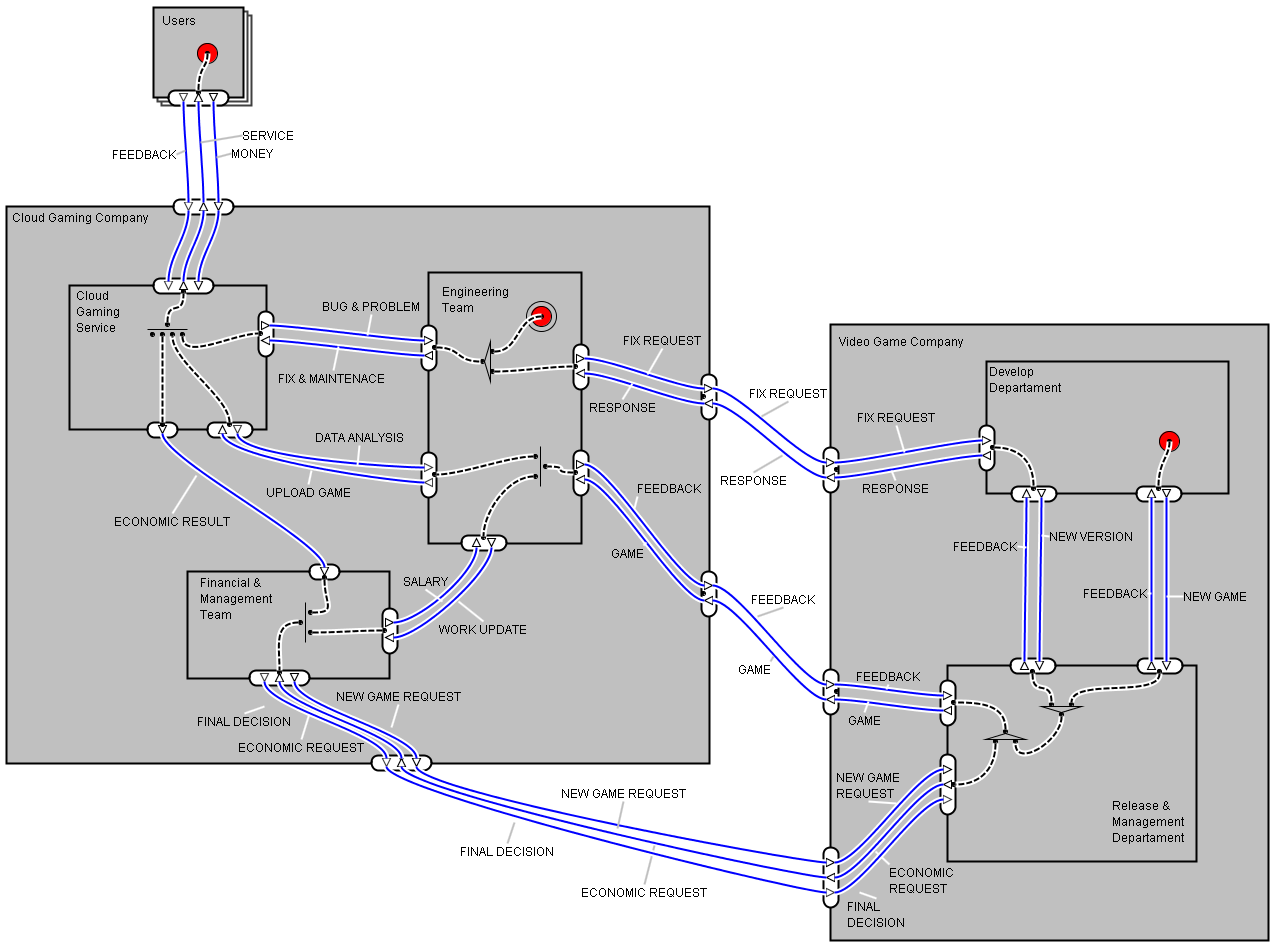
\includegraphics[scale=0.45]{value_model}
\caption{Value Diagram}
\label{Value Diagramn }
\end{figure} 

\chapter{Business Evaluation}
In this part of the project, assumptions were made about what the evaluation criteria of the above-mentioned business might be. \\
In fact, it was intended to hypothesize some factors such as Critical Successor Factors, Key goal Indicators, and Key performace Inficators. \\
All these factors were calculated hypothetically as we do not have any real data related to a cloud gaming service. \\
The purpose of this section is to show a pontential analysis that could be applied in a real-world context. 
\section{Critical Successor Factors (CSF)}
Critical success factors (CSFs) are critical factors or activities that can evaluate the success of the company. In our case study, we can denote as CSFs:
\begin{itemize}
\item{\textbf{Number of subscribed users:} the higher the number of subscribed users, the higher the revenue of the cloud service and consequently the more budget is available to buy and have new games produced }
\item{\textbf{Number of hours per user on the platform:} the more a user uses the platform the more it means they are satisfied, this could ensure a prolonged subscription over time.  }
\item{\textbf{Number of shares by the user:} for example, sharing on social networks, which could lead more users to subscribe.}
\item{\textbf{Number of platform disservices:} the lower the number of reports on platform operation, the higher the level of satisfaction increases}
\end{itemize}
\newpage
\section{Key Goal Indicators}
Key Goal Indicators (KGI) define the metrics to check whether the company's goal has been achieved. 
For example, they are useful goals for quantifying business progress. In our case we can define:
\begin{itemize}
\item{\textbf{New subscribers:} the steady increase in the number of users subscribing to the service ensures that the company can grow. }
\item{\textbf{Growth in service use:} users are using the platform more often ensures continued service growth.}
\item{\textbf{Increased sharing by users:} Increase users' sharing of content on social platforms to gain more visibility and active users } 
\item{\textbf{Reduce disservices on platform:} the lower the number of reports on platform operation, the higher the level of satisfaction increases}
\end{itemize}
\section{Key Performance Indicators}
Key Performance Indicators (KPIs) are an index that express what you want to
achieve by when. They are the quantifiable, outcome-based statements you’ll use to measure if
you’re on track to meet your goals or objectives.
KPIs are used to measure the results achieved by the organization.\\ In the case we can define:
\begin{itemize}
\item{\textbf{Rate of new subscribed users:} Number of new users who subscribe to the system in a defined time ( i.e. daily, monthly... ) }
\item{\textbf{Average time on the platform:} Average time spent within the platform by users  }
\item{\textbf{Average of monthly accesses:} Average of monthly accesses by a subscribers users on the platform  }
\item{\textbf{Number of monthly shares by the users:} Number of sharing on social networks, which could lead more users to subscribe.}
\item{\textbf{Number of platform disservices:} The value is the number of daily reports made by users.}

\end{itemize}

\section{KPI in Practice}

\begin{figure}[H]
 \centering
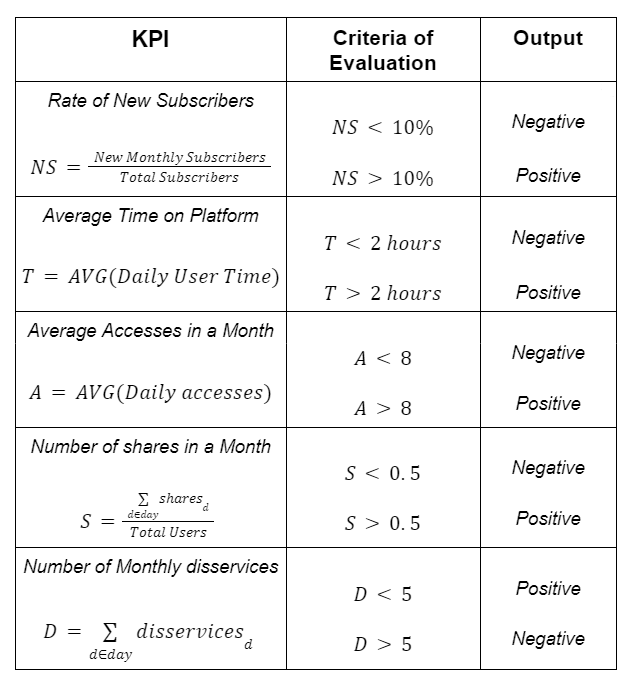
\includegraphics[scale=0.8]{KPI}
\caption{KPI evaluation}
\label{KPi }
\end{figure} 


\chapter{Implementation on AWS}
In this chapter will be implemented a possible solution of a cloud gaming platform on AWS.\\\\
AWS stands for Amazon Web Services, which is a cloud computing platform provided by Amazon. AWS offers a wide range of cloud-based services, including computing power, database storage, content delivery, and other functionality to help businesses scale and grow. The platform provides flexible, scalable, and cost-effective cloud computing solutions for businesses of all sizes, from startups to large enterprises. With AWS, users can quickly provision resources and scale their infrastructure as needed, paying only for what they use.\\\\
In particular, in this section will be delve into the various components that are used to build this platform and their purpose.\\
The entire architecture will be serverless meaning that a model of software design and deployment that eliminates the need for server infrastructure management by the developer. In a serverless architecture, the cloud provider takes responsibility for managing the infrastructure and running the server, allowing the developer to focus on writing code. This approach is also referred to as Function-as-a-Service (FaaS), where functions are invoked in response to events triggered by user actions or system events. The main benefit of a serverless architecture is that it eliminates the need for upfront infrastructure investment, enabling rapid scaling and reducing operational costs.
%
\begin{figure}[H]
 \centering
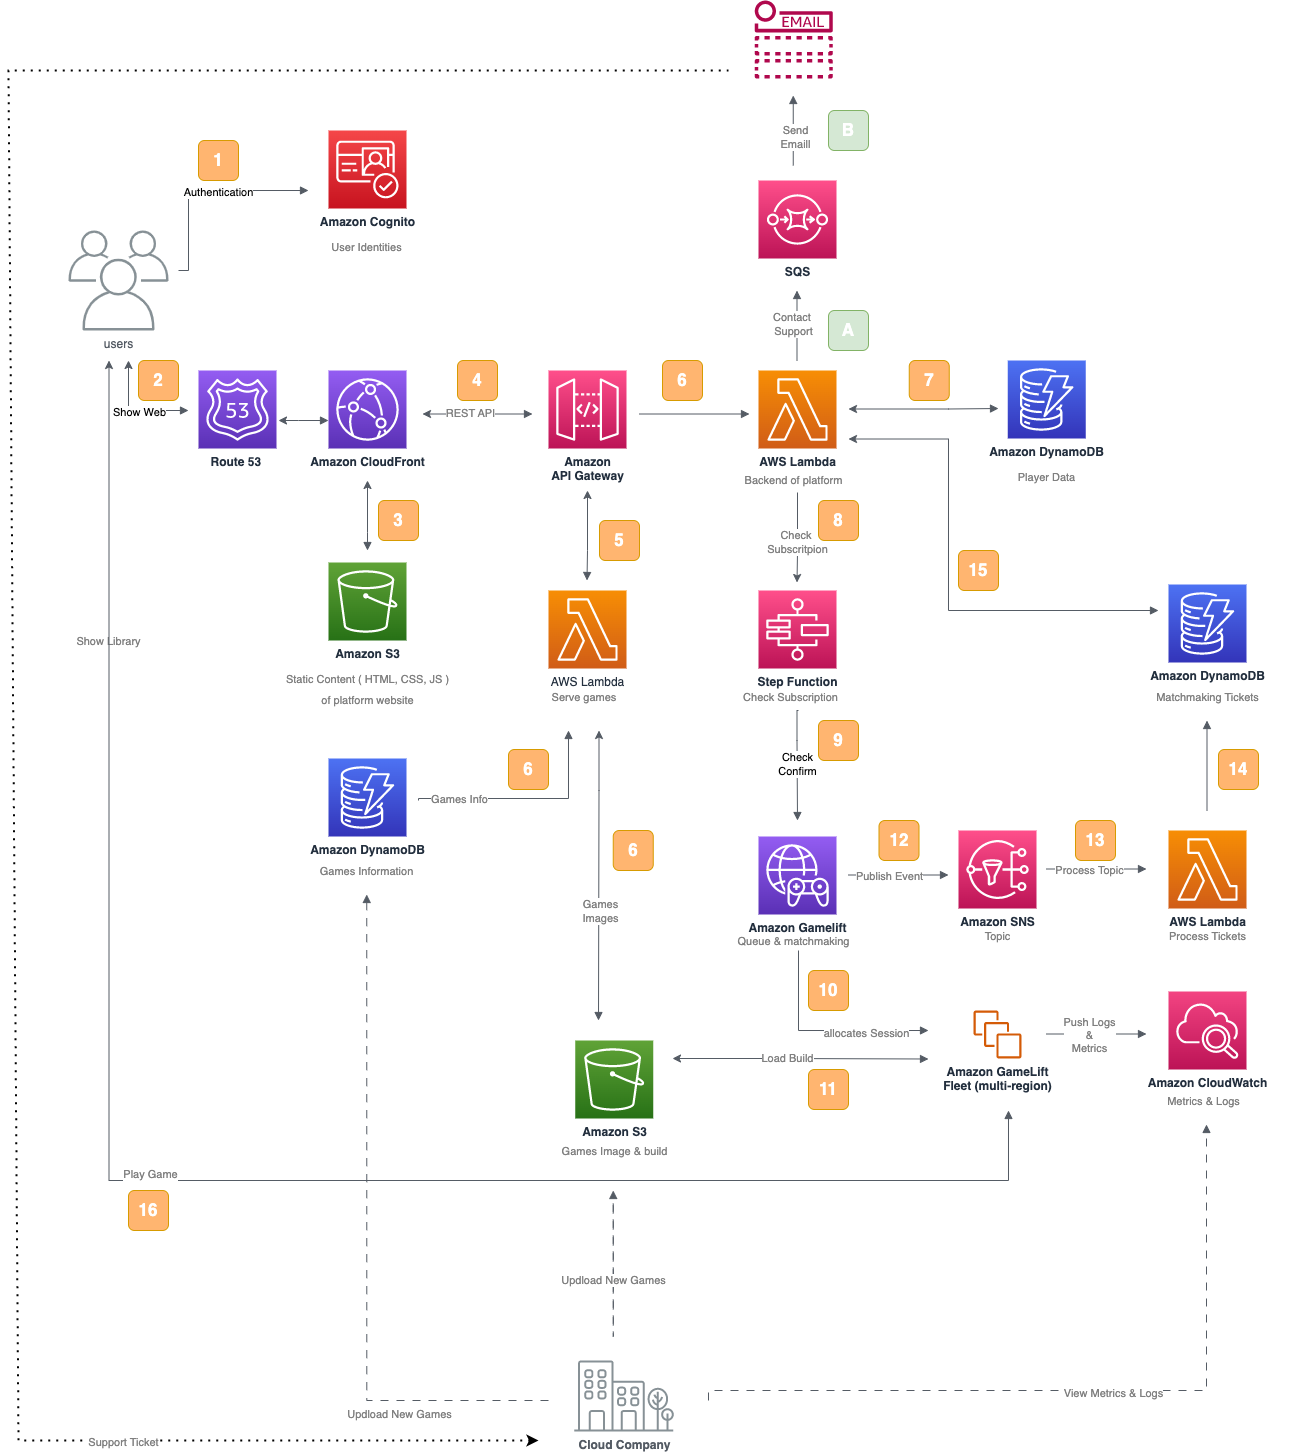
\includegraphics[scale=0.35]{img/AWS_BPMN}
\caption{Architecture Diagram}
\label{AWS Architecture Diagram }
\end{figure} 
\section{AWS Work Flow}
This implementation demonstrates a potential architecture for a cloud gaming platform. Users can register or log in using AWS Cognito. DNS linking and request balancing are managed by Route 53 and CloudFront. S3 enables access to the game library via CloudFront, while API Gateway, combined with Lambda, creates a REST API for accessing game files, player data, raising support team requests, or initiating a game session. If a game session is initiated, Step Functions orchestrate the possible subscription control. If there is no subscription, Step Functions direct the user to subscribe. If there is already an active subscription, Gamelift is utilized to initiate the game. Gamelift manages all game aspects, including resource provisioning, user queues, finding users with similar game characteristics, and more. CloudWatch monitors any issues, logs, and displays information on a dashboard for the company.
\section{AWS Services}

%
\begin{wrapfigure}{r}{0.25\textwidth}
  \centering
  
\includegraphics[width=0.2\textwidth]{img/services/cognito}
\end{wrapfigure}
%
%
\paragraph{Amazon Cognito} is a product that provides user authentication, authorization, and user management services to web and mobile applications. It is designed to provide a simple and secure way for developers to add user sign-up, sign-in, and access control to their applications.\\
With Amazon Cognito the users can do sign-up and sign-in on the platform. It also supports user authentication with popular third-party identity providers such as Facebook, Google, and Amazon, making it easy for users to sign up and sign in to applications with their existing social media accounts.\\\\
%
%
%
\begin{wrapfigure}{l}{0.25\textwidth}
  \centering
  
\includegraphics[width=0.2\textwidth]{img/services/Route-53}
\end{wrapfigure}
%
\paragraph{Amazon Route 53} is a highly scalable and reliable Domain Name System (DNS) service offered by Amazon Web Services (AWS). It provides a way to route traffic for domains to different AWS resources.\\
Route 53 also provides features like DNS failover, health checks, latency-based routing, and geo DNS. These features enable users to create highly available and fault-tolerant systems that can withstand infrastructure failures and traffic spikes.\\
With Amazon Route 53 manages DNS resolution and the routing of web traffic generated by users worldwide.\\\\
%
%
%
\begin{wrapfigure}{r}{0.25\textwidth}
  \centering
  
\includegraphics[width=0.2\textwidth]{img/services/CloudFront}
\end{wrapfigure}
%
\paragraph{Amazon CloudFront} is a content delivery network (CDN) service provided by Amazon Web Services (AWS). It delivers content, including web pages, videos, and other types of digital media, from AWS edge locations worldwide to end-users.\\
CloudFront is designed to improve the performance, security, and availability of web applications and content by caching content at edge locations close to end-users. This reduces latency and minimizes the load on the origin server.\\\\
CloudFront is a powerful CDN service that helps improve the performance, security, and scalability of web applications and content delivery for this reason it plays a crucial role in managing the content required by users by being positioned ahead of the web platform's API to improve the performance of requests.\\\\
%
%
%
\begin{wrapfigure}{l}{0.25\textwidth}
  \centering
  
\includegraphics[width=0.2\textwidth]{img/services/S3}
\end{wrapfigure}
%
\paragraph{Amazon S3}  is a cloud-based object storage service provided by AWS. It provides a scalable and secure platform for storing and retrieving data, such as images, videos, documents, and other types of digital files.\\
S3 provides high durability, availability, and security of data, achieved by automatically replicating data across multiple geographically distributed data centers and providing strong security controls, such as encryption in transit and at rest.\\
S3 supports a wide range of use cases, from simple storage and retrieval of files to more complex workflows involving data processing, backup and archival, content distribution, and website hosting. It provides different storage classes to meet different requirements, such as standard storage for frequently accessed data, infrequent access storage for less frequently accessed data, and archive storage for long-term data retention.\\
S3 integrates with other AWS services, such as AWS Lambda, Amazon CloudFront and ensure high  scalable and high-performance applications quickly and easily. In this particular case, it was utilized for storing game files, such as images, videos, and builds. Additionally, it provides a user-friendly web interface for integrating the web platform library, where users can easily select their preferred games.\\\\
%
%
%
\begin{wrapfigure}{r}{0.25\textwidth}
  \centering
  \includegraphics[width=0.2\textwidth]{img/services/API-Gateway}
\end{wrapfigure}
%
\paragraph{Amazon API Gateway} is a fully managed service provided by AWS that makes it easy to create, deploy, and manage APIs at any scale. With API Gateway, can create APIs that act as a front door for applications to access data, business logic, or functionality from backend services like in this case Backend logic from AWS Lambda,but it could works with other any HTTP endpoint.\\
%
API Gateway handles all the tasks involved in securely accepting and processing API requests, including traffic management, authorization and access control, monitoring and analytics, and API version management. It supports a range of API protocols, including RESTful APIs and WebSocket APIs, and provides several options for integrating with backend services, such as Lambda functions and HTTP/HTTPS endpoints.\\
%
In this scenario,  when a user requests a game, API Gateway can handle the task of calling the backend application through the use of APIs. It is particularly powerful when linked to AWS Lambda, which can manage all of the logic for the web platform. With API Gateway, developers can easily manage the entire process of securely accepting and processing API requests, including traffic management, authorization, monitoring, and API version management. \\\\
%
%
%
\begin{wrapfigure}{l}{0.25\textwidth}
  \centering
  
\includegraphics[width=0.2\textwidth]{img/services/Lambda}
\end{wrapfigure}
%
\paragraph{Amazon Lambda} is a serverless compute service provided by AWS that allows to run code in response to events or triggers, without the need to provision or manage servers. With Lambda, can upload their code in the form of a function and define the events or triggers that will invoke that function. Lambda is a fully managed service, which means that AWS handles all aspects of the infrastructure management, security, and availability of the service, allowing developers to focus on writing code and building applications.\\
Lambda functions can be triggered by a wide range of event sources, including HTTP requests through API Gateway, file uploads to Amazon S3, messages sent to Amazon SNS or Amazon SQS, changes in data stored in Amazon DynamoDB or integrates with step function. All these possibility were used in this project in several Lambda functions.\\
Specifically, one Lambda function was used to retrieve game information from DynamoDB and images and build games from S3 after an API call. Another Lambda function was used to retrieve player data from DynamoDB, manage SQS in case of problem reporting, and integrate with Step Functions to manage the flow before starting the game. Finally, another Lambda function was used to manage matchmaking during the game.\\\\
%
%
%
\begin{wrapfigure}{r}{0.25\textwidth}
  \centering
  
\includegraphics[width=0.2\textwidth]{img/services/DynamoDB}
\end{wrapfigure}
%
\paragraph{Amazon DynamoDB} is a fully managed NoSQL database service provided by AWS. It is designed to provide fast and flexible storage for applications that require low latency and high scalability.  It supports key-value and document data models, which allows developers to choose the most appropriate data model for their application.\\
DynamoDB is a highly available and durable service that automatically replicates data across multiple Availability Zones to ensure data durability and availability this features are perfect for this specific use case. It also provides built-in security features, such as encryption at rest and in transit, to help protect user data.\\
DynamoDB played a crucial role in this project by providing a storage solution for game information, player data, and matchmaking. This component was particularly important as it significantly improved the application's speed and overall user experience.\\\\
%
%
%
\begin{wrapfigure}{l}{0.25\textwidth}
  \centering
  
\includegraphics[width=0.2\textwidth]{img/services/Step-Functions}
\end{wrapfigure}
%
\paragraph{Amazon Step Functions}  is a serverless workflow service provided by AWS that allows developers to coordinate distributed applications and microservices using visual workflows. It enables the creation of serverless workflows that integrate with other AWS services and third-party APIs, enabling the creation of complex, long-running workflows.
Step Functions provides a visual interface for designing and orchestrating workflows. It used to define the sequence of steps, conditional logic, and error handling for each step in the workflow. \\
In this scenario, the payment process is orchestrated using Step Functions. A defined workflow is utilized to check whether the user is subscribed or not. If the user is subscribed, they will be permitted to proceed and play the game. On the other hand, if the user is not subscribed, they will be required to subscribe before they can play on the platform.\\\\
%
%
\begin{wrapfigure}{r}{0.25\textwidth}
  \centering
  
\includegraphics[width=0.2\textwidth]{img/services/GameLift}
\end{wrapfigure}
%
\paragraph{Amazon Gamelift} is a managed service offered by AWS that enables developers to deploy, operate, and scale dedicated game servers in the cloud. GameLift provides tools to manage sessions, players, and scaling capacity based on game traffic. It supports both real-time multiplayer games and games with a large number of concurrent players. With GameLift, developers can focus on creating great gameplay experiences while AWS manages the infrastructure required to run dedicated game servers at scale.\\\\ 
In this example, Amazon GameLift resources are utilized to host game servers and matchmaking functionality.GameLift FlexMatch publishes an event to Amazon SNS on matchmaking success.\\ The deployment includes the following components:
\begin{itemize}
\item \textbf{FlexMatch Matchmaking} rule set, which defines players based on their experience, play hours, and skill levels. This information is stored in the backend service using DynamoDB.The FlexMatch rule set also specifies a latency threshold to reduce the occurrence of lags.

\item \textbf{FlexMatch matchmaking configuration} utilizes the rule set and directs game session placement requests to the queue.

\item \textbf{GameLift Queue} is responsible for placing game sessions on the GameLift Fleet. The example features a single fleet behind the queue, which is located in two regional locations (home region and one secondary region).

\item \textbf{GameLift Fleet}, located behind the queue, employs the latest game server build and runs on Amazon Linux 2. It has two regional locations and each instance runs two game server processes. Depending on the instance size and resource requirements of the game server, more game servers can be packed onto each instance.
\end{itemize}
\newpage


%
%
%
\begin{wrapfigure}{l}{0.25\textwidth}
  \centering
  
\includegraphics[width=0.2\textwidth]{img/services/SNS}
\end{wrapfigure}
%
\paragraph{Amazon Amazon Simple Notification Service} or SNS is a fully managed messaging service provided by AWS. It enables the creation, publishing, and distribution of messages to a large number of subscribers or other distributed services.\\
SNS operates on a publish/subscribe model, where publishers send messages to SNS topics, and subscribers receive messages from those topics. Topics can be thought of as communication channels that group together messages of similar interest, such as notifications for a specific application or alerts for a particular event.
In this scenario, Amazon Simple Notification Service (SNS) is utilized to initiate the execution of a subscribed AWS Lambda function for ticket processing. SNS acts as a messaging service that facilitates the distribution of messages or events to a Lambda function subscribed to a specific topic.
When a message is published to an SNS topic, all the subscribed Lambda functions are triggered to execute their associated code. This event-driven architecture allows the Lambda function to be invoked in response to the published message, ensuring that the relevant processing takes place.\\\\
%
%
%
\begin{wrapfigure}{r}{0.25\textwidth}
  \centering
  
\includegraphics[width=0.2\textwidth]{img/services/SQS}
\end{wrapfigure}
%
\paragraph{Amazon Simple Queue Service} or SQS is a fully managed message queuing service provided by AWS. It enables decoupling of components and distributed systems by allowing messages to be sent, stored, and retrieved asynchronously between different software components, systems, or services.
SQS operates on a simple queue model, where messages are placed in a queue and then retrieved by one or more consumer components, which may be running on separate systems or instances. SQS provides a reliable and scalable infrastructure that ensures that messages are stored safely and that they are only delivered once.\\
SQS supports two types of queues: Standard and FIFO. Standard queues provide at-least-once delivery guarantee and are designed for high throughput, where ordering of messages is not critical. FIFO queues provide first-in-first-out delivery and ordering of messages is guaranteed, making them ideal for scenarios where sequencing and deduplication of messages are important, such as financial transactions or workflow processing. Second kind of SQS it was used on this project for manage the report problem. In this project, the second type of Amazon SQS was utilized for efficient management of reported issues. Specifically, users were able to notify the support team of any platform or game bugs by sending an email to a dedicated email address.\\\\

%
%
%
\begin{wrapfigure}{l}{0.25\textwidth}
  \centering
  
\includegraphics[width=0.2\textwidth]{img/services/CloudWatch}
\end{wrapfigure}
%
\paragraph{Amazon CloudWatch} is a monitoring and observability service provided by AWS that allows users to collect, monitor, and analyze various metrics, logs, and events from AWS resources, applications, and services. CloudWatch provides a unified view of an organization's cloud resources and applications, enabling them to gain insights into their operational health and performance, troubleshoot issues, and optimize resource utilization.\\
CloudWatch supports monitoring of various metrics, such as CPU utilization, network traffic, and storage capacity, for EC2 instances, databases, load balancers, and other AWS resources. Additionally, CloudWatch can also collect logs and events from various sources, such as AWS Lambda functions, API Gateway, and CloudTrail, allowing users to analyze and troubleshoot issues in real-time.\\
CloudWatch provides a variety of features, including dashboards, alarms, and automated actions, that enable users to proactively monitor and respond to changes in their resources or applications. Users can create customizable dashboards to visualize their metrics and logs, set alarms to notify them of critical events or changes, and configure automated actions, such as scaling resources, based on certain thresholds or patterns.
In this project, this particular component played a crucial role in monitoring all aspects of the platform by collecting and providing comprehensive information.\\\\
%
%

\chapter{Conclusion}
In conclusion, this new technology will evolve in the future and make it more accessible to play from any device without the need for high performance. 
In this project, we wanted to represent a model of how the company would operate in order to identify the factors necessary for growth.\\
Although the entire drafting was based on a hypothetical structure of a cloud gaming service company it was possible to represent in detail all process steps and business-side evaluation criteria. In particular, the BPMN diagram and the Value Model diagram made it possible to show the unfolding of the process and to illustrate in a simple and intuitive way all the stages of developing and enjoying a video game on a cloud platform.\\
Through CSFs, KGIs the KPIs it is possible to evaluate better strategies to achieve greater profits and reach as many people as possible.\\\\
%
As mentioned above unfortunately there was no real data available especially concerning the evaluation criteria that each company uses to define a business strategy, nevertheless it was possible to simulate a hypothetical case study in which a real company that uses this type of service could be placed. \\\\
%
%
Chapter 6 of this project was focused on exploring how the architecture could be implemented on AWS. Although the specific architecture presented is not a deployed or tested solution, the goal of this chapter was to demonstrate that it is possible to create a functional cloud gaming platform using AWS services. The chapter provided an overview of the key AWS services that could be used to build the platform, and outlined how they could be integrated to create a cohesive system. While additional components or configuration details may be required for a real-world deployment, the architecture presented in this chapter serves as a starting point for anyone looking to build a cloud gaming platform on AWS. 


\end{document}


 
